\section{Complex numbers}

The foundation of the \textit{complex numbers} is given by the imaginary unit \(i\), defined either as \(i = \sqrt{-1}\) or as \(i^2 = -1\).

A complex number \(z\) can be written as \(a + bi\), where \(a, b \in \mathbb{R}\). The real numbers \(a\) and \(b\) are known as the \textit{real part} and the \textit{complex part} of \(z\) respectively.

The set of all complex numbers is denoted as \(\mathbb{C}\). Note that the set of real numbers \(\mathbb{R}\) is a subset of \(\mathbb{C}\). See figure \ref{fig:Ch01-reals-in-complex}.


\begin{figure}[H]
    \centering
    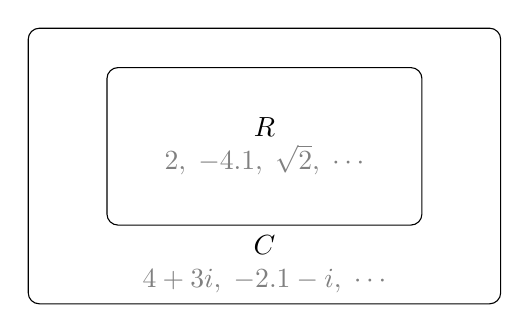
\begin{tikzpicture}
        \draw[rounded corners] (-2,0) rectangle (2,-2);

        \draw[rounded corners] (-3,0.5) rectangle (3,-3);

        \node[align=center] at (0,-1)  {\(\mathbb{R}\)\\ {\color{gray} \(2,\; -4.1,\; \sqrt{2},\; \cdots\)}};

        \node[align=center] at (0,-2.5)  {\(\mathbb{C}\)\\ {\color{gray} \(4+3i,\; -2.1-i,\; \cdots\)}};
    \end{tikzpicture}
    \caption{The set of real numbers \(\mathbb{R}\) is a subset of the set of complex numbers \(\mathbb{C}\). All real numbers are complex numbers.}
    \label{fig:Ch01-reals-in-complex}
\end{figure}





\subsection{Basic arithmetic with complex numbers, and complex conjugates}

To add or subtract two complex numbers, we deal with the real and imaginary parts separately.
%
\begin{align*}
    (2+3i) + (5-8i) &= (2+5) + (3 + (-8))i = 7 - 5i \tag{Addition}\\
    (2+3i) - (5-8i) &= (2-5) + (3 - (-8))i = -3 + 11i \tag{Subtraction}
\end{align*}

The multiplication of complex numbers is also straightforward as long as we bear in mind that \(i^2 = -1\).
%
\begin{align*}
    (3 + 4i)(-2 + 3i) &= -6 + 9i - 8i + 12i^2\\
    &= (-6-12) + (9-8)i\\
    &= -18 + i
\end{align*}

To divide a complex number by another, e.g.
%
\[\frac{a+bi}{c+di}\]
%
we multiply both the numerator and denominator by \(c - di\), which is obtained by flipping the sign of the imaginary part of the denominator. For example, if we want to compute
%
\[\frac{2+3i}{5-4i}\text{,}\]
%
we flip the sign of the imaginary part of \(5 - 4i\) to get \(5 + 4i\). We then multiply both the numerator and denominator of the fraction by this \(5 + 4i\) to get
%
\begin{align*}
    \frac{2+3i}{5-4i} &= \frac{(2+3i)(5 + 4i)}{(5-4i)(5 + 4i)}\\
    &= \frac{10 + 8i + 15i - 12}{25 + 20i - 20i + 16}\\
    &= \frac{-2 + 23i}{41}\\
    &= \frac{-2}{41} + \frac{23}{41}i \text{.}
\end{align*}

Notice how multiplying \(5 - 4i\) with \(5 + 4i\) produces the real number \(41\). By flipping the sign of the imaginary part of a complex number, we obtain what's called its \textit{complex conjugate}. The complex conjugate of \(z\) is denoted as \(\overline{z}\). By writing \(z\) as \(a + bi\), we can easily prove that the product of any complex number with its conjugate must equal a real number:
%
\[z \times \overline{z} = (a + bi)(a - bi) = a^2 + b^2 \in \mathbb{R}\text{.}\]





\subsection{Visualising complex numbers}

Given some complex number \(z = x + yi\), we can treat its real and imaginary parts as Cartesian coordinates, thus mapping it to a point on the 2D plane.

\begin{figure}[H]
    \centering

    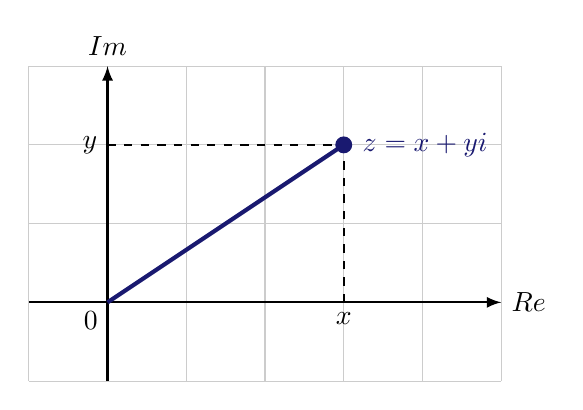
\begin{tikzpicture}
        \draw[thin,gray!40] (-1,-1) grid (5, 3);
        \draw[thick, ->, >=latex] (-1,0)--(5,0) node[right]{\(\mathfrak{Re}\)};
        \draw[thick, ->, >=latex] (0,-1)--(0,3) node[above]{\(\mathfrak{Im}\)};
        \draw (0, 0) node[below left] {\(0\)};
        
        \draw[dashed, thick] (3, 0) node[below]{\(x\)} --(3, 2);
        \draw[dashed, thick] (0, 2) node[left]{\(y\)} --(3, 2);

        \filldraw[radius=0.1, MidnightBlue] (3,2) circle;
        \draw[line width=1.5pt, MidnightBlue] (0,0)--(3,2) node[anchor=west]{\(\;z = x + yi\)};
    \end{tikzpicture}
    
    \caption{The complex number \(z = x + yi\) as a point on the 2D plane}
    \label{fig:02-ket-3-1}
\end{figure}



\subsection{Exponential form}

Recall that it is possible to express a point on a 2D plane using polar coordinates \((R, \theta)\) as well. Indeed, given any complex number \(z = x+yi\), we can find its corresponding pair of values \(R\) and \(\theta\).

\begin{figure}[H]
    \centering

    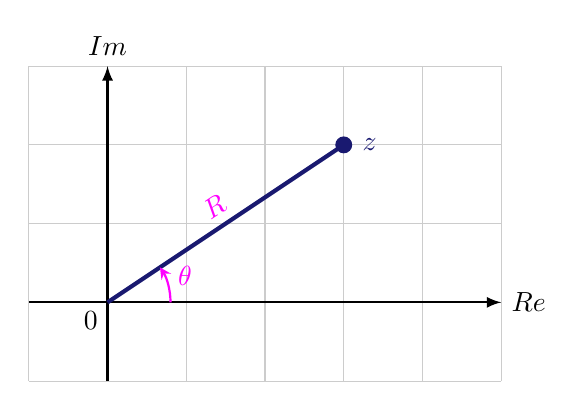
\begin{tikzpicture}
        \draw[thin,gray!40] (-1,-1) grid (5, 3);
        \draw[thick, ->, >=latex] (-1,0)--(5,0) node[right]{\(\mathfrak{Re}\)};
        \draw[thick, ->, >=latex] (0,-1)--(0,3) node[above]{\(\mathfrak{Im}\)};
        \draw (0, 0) node[below left] {\(0\)};

        \filldraw[radius=0.1, MidnightBlue] (3,2) circle;
        \draw[line width=1.5pt, MidnightBlue] (0,0)--(3,2) node[pos=0.5, sloped, anchor=south, Fuchsia]{\(R\)} node[anchor=west]{\(\;z\)};
        \draw[-stealth,Fuchsia, thick] (0.8, 0) arc (0:33.69:0.8) node[pos=0.5, anchor=west, shift={(0, 0.1)}]{\(\theta\)};
    \end{tikzpicture}
    
    \caption{The position of a complex number on the 2D plane can be represented using polar coordinates.}
    \label{fig:Ch01-complex-num-polar}
\end{figure}

Based on this idea, we introduce a new notation as follows.
%
\begin{quote}
    If the position of a complex number \(z\) on the 2D plane can be represented by the polar coordinates \((R, \theta)\), then we have
    %
    \[z = R \times e^{i\theta}\]
    %
    where \(R, \theta \in \mathbb{R}\) and \(R \geq 0\).

    \(R\) is called the \textit{absolute value} or \textit{modulus} of \(z\) and is denoted as \(\abs{z}\). This represents the point's position from the origin.

    \(\theta\) is called the \textit{argument} of \(z\) and is denoted as \(\arg(z)\). This represents the angle from horizontal.
\end{quote}
%
This way of representing complex numbers is known as the \textit{exponential form}. (This is a natural result of Euler's formula \(e^{i\theta} = \cos{\theta} + i\sin{\theta}\).)

Now consider two complex numbers expressed in exponential form.
%
\begin{align*}
    z_1 &= R_1 \times e^{i\theta_1}\\
    z_2 &= R_2 \times e^{i\theta_2}
\end{align*}
%
These two numbers are considered equal if both of the following conditions hold.
%
\begin{align*}
    R_1 &= R_2\\
    \theta_1 &= \theta_2 {\;\color{BrickRed} +2k\pi} \tag{for some \(k \in \mathbb{Z}\)}
\end{align*}
%
Note that the red part is necessary because a rotation of \(2\pi\) radians has no effect on a point's position.

The exponential form makes the multiplication and division of complex numbers a lot easier.

\begin{tabular}{c|c}
    \textbf{Multiplication} & \textbf{Division}\\
    \parbox{0.5\textwidth}{\centering
        \begin{align*}
            (1 \times e^{\frac{\pi}{6} i}) \times (2 \times e^{-\frac{\pi}{4} i}) &= 2 \times e^{\frac{\pi}{6} i -\frac{\pi}{4} i}\\
            &= 2 \times e^{-\frac{\pi}{12} i}
        \end{align*}
    }
    &
    \parbox{0.5\textwidth}{\centering
        \begin{align*}
            \frac{1 \times e^{\frac{\pi}{6} i}}{2 \times e^{-\frac{\pi}{4} i}} &= \frac{1}{2} \times \frac{e^{\frac{\pi}{6} i}}{e^{-\frac{\pi}{4} i}}\\
            &= 2 \times e^{\frac{5\pi}{12} i}
        \end{align*}
    }
\end{tabular}




\subsection{Converting between Cartesian and exponential forms}

The methods used to convert between the Cartesian form \(x + yi\) and the exponential form \(R \times e^{i\theta}\) are outlined below.
%
\begin{itemize}
    \item \textbf{Given the Cartesian form of a complex number, find its exponential form.}

    Given the Cartesian form \(z = x+yi\), we can find the modulus using Pythagoras' theorem.
    %
    \[\abs{z} = \sqrt{x^2 + y^2}\]
    %
    The argument can be found using the arctangent.
    %
    \[\arg(z) = \arctan\left(\frac{y}{x}\right)\]

    \item \textbf{Given the exponential form of a complex number, find its Cartesian form.}

    Given the exponential form \(z = R \times e^{i\theta}\), we can find the Cartesian coordinates using simple trigonometry.
    %
    \begin{align*}
        x &= R \cos{\theta}\\
        y &= R \sin{\theta}
    \end{align*}
\end{itemize}

To speed up conversion processes, it is often useful to memorize the Cartesian coordinates of some special points on the unit circle. See figure \ref{fig:Ch01-cartesian-coords-on-unit-circle} and table \ref{tab:Ch01-classic-angle-trig}.

\begin{figure}[H]
    \centering
    \includegraphics[width=0.6\linewidth]{Images/CartesianCoordsOnCircle.png}
    \caption{It is important to know the coordinates of points on the circle corresponding to classic angles.}
    \label{fig:Ch01-cartesian-coords-on-unit-circle}
\end{figure}

\begin{table}[H]
    \centering
    \begin{tabular}{|c||c|c|c|}
        \hline
        \(\theta\) (radians) & \(\pi/6\) & \(\pi/4\) & \(\pi/3\) \\
        \hline
        \(\theta\) (degrees) & \(30\degree\) & \(45\degree\) & \(60\degree\) \\
        \hline
        \(\sin{\theta}\) & \(\dfrac{1}{2}\) & \(\dfrac{\sqrt{2}}{2}\) & \(\dfrac{\sqrt{3}}{2}\)\\[1.5ex]
        \hline
        \(\cos{\theta}\) & \(\dfrac{\sqrt{3}}{2}\) & \(\dfrac{\sqrt{2}}{2}\) & \(\dfrac{1}{2}\)\\[1.5ex]
        \hline
    \end{tabular}
    \caption{The values of \(\sin{\theta}\) and \(\cos{\theta}\) for some classic angles \(\theta\).}
    \label{tab:Ch01-classic-angle-trig}
\end{table}




\subsection{Visualising arithmetic on complex numbers}

When visualised on the 2D plane, the addition of complex numbers is similar to that of vectors. We join the arrows in a tip-to-tail manner in order to determine the sum, as shown in figure \ref{fig:Ch01-adding-complex-numbers}.


\begin{figure}[H]
    \centering

    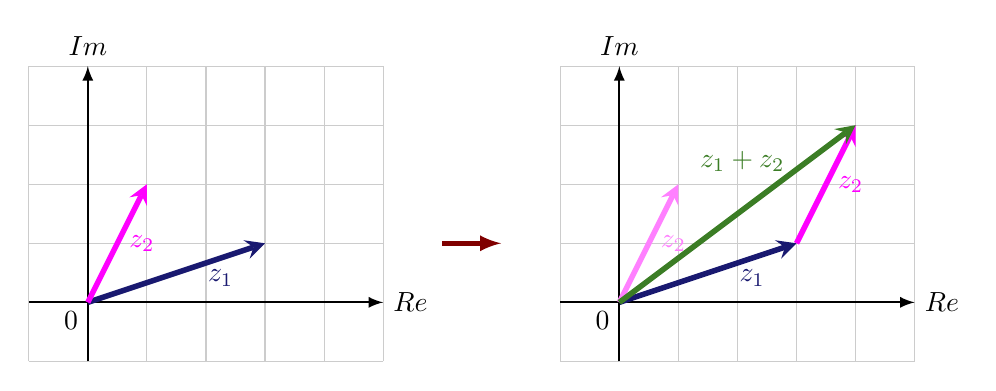
\begin{tikzpicture}[scale=0.75]
        \draw[thin,gray!40] (-1,-1) grid (5, 4);
        \draw[thick, ->, >=latex] (-1,0)--(5,0) node[right]{\(\mathfrak{Re}\)};
        \draw[thick, ->, >=latex] (0,-1)--(0,4) node[above]{\(\mathfrak{Im}\)};
        \draw (0, 0) node[below left] {0};
        
        \draw[line width=2pt, MidnightBlue, -stealth] (0,0)--(3,1) node[pos=3/4, below]{\(z_1\)};
        \draw[line width=2pt, Fuchsia, -stealth] (0,0)--(1,2) node[pos=1/2, anchor=west]{\(z_2\)};

        \draw[ultra thick, Maroon, ->, >=latex] (6, 1)--(7, 1);
        
        \begin{scope}[shift={(9, 0)}]
            \draw[thin,gray!40] (-1,-1) grid (5, 4);
            \draw[thick, ->, >=latex] (-1,0)--(5,0) node[right]{\(\mathfrak{Re}\)};
            \draw[thick, ->, >=latex] (0,-1)--(0,4) node[above]{\(\mathfrak{Im}\)};
            \draw (0, 0) node[below left] {0};
            
            \draw[line width=2pt, MidnightBlue, -stealth] (0,0)--(3,1) node[pos=3/4, below]{\(z_1\)};
            \draw[line width=2pt, Fuchsia!50, -stealth] (0,0)--(1,2) node[pos=1/2, anchor=west]{\(z_2\)};
            \draw[line width=2pt, Fuchsia, -stealth] (3,1)--(4,3) node[pos=1/2, anchor=west]{\(z_2\)};

            \draw[line width=2pt, OliveGreen, -stealth] (0,0)--(4,3) node[pos=3/4, anchor=east, shift={(0, 0.1)}]{\(z_1+z_2\)};
        \end{scope}
        
    \end{tikzpicture}
    
    \caption{Addition of complex numbers.}
    \label{fig:Ch01-adding-complex-numbers}
\end{figure}

The above figure also illustrates another key idea. Notice how in the figure on the right, the vectors of \(z_1\), \(z_2\) and \(z_1 + z_2\) form a triangle. This means their absolute values must fulfil the triangle inequality.
%
\[\abs{z_1} + \abs{z_2} \geq \abs{z_1+z_2}\]

To visualise multiplication we consider the exponential form. As shown in figure \ref{fig:Ch01-multiplying-complex-numbers}, when two complex numbers are multiplied, their arguments are added together to produce a rotation, while their moduli are multiplied.


\begin{figure}[H]
    \centering

    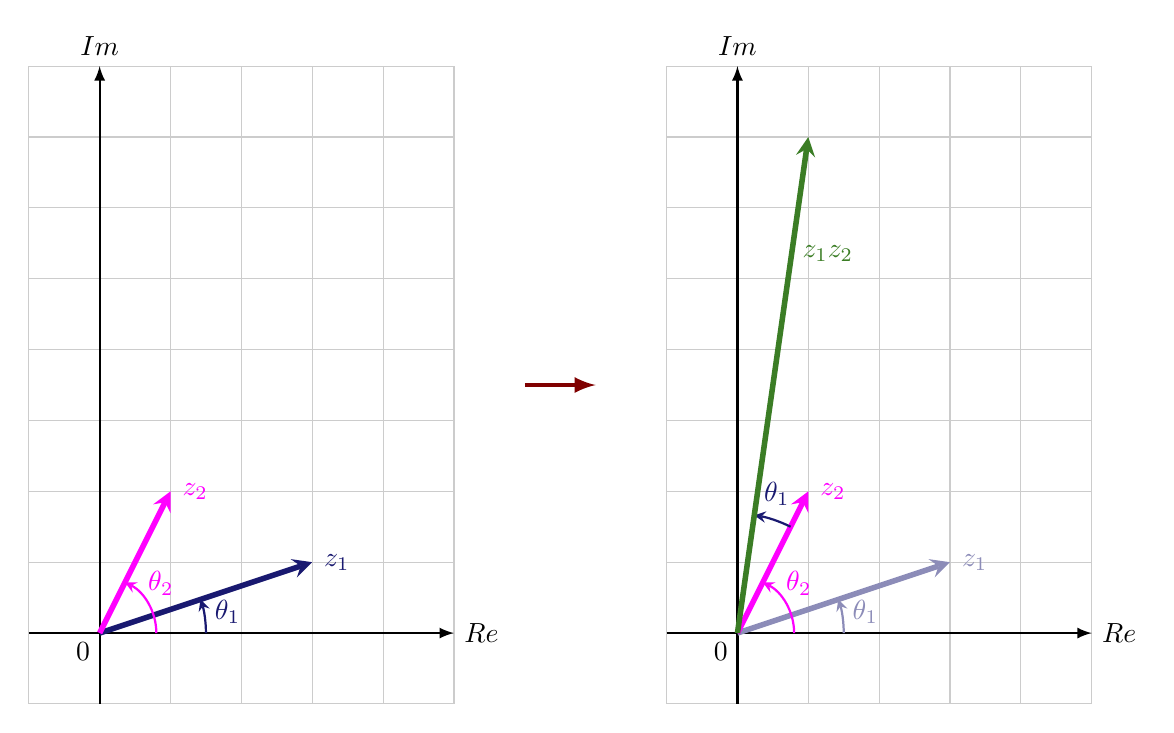
\begin{tikzpicture}[scale=0.9]
        \draw[thin,gray!40] (-1,-1) grid (5, 8);
        \draw[thick, ->, >=latex] (-1,0)--(5,0) node[right]{\(\mathfrak{Re}\)};
        \draw[thick, ->, >=latex] (0,-1)--(0,8) node[above]{\(\mathfrak{Im}\)};
        \draw (0, 0) node[below left] {0};
        
        \draw[line width=2pt, MidnightBlue, -stealth] (0,0)--(3,1) node[right]{\(z_1\)};
        \draw[-stealth, MidnightBlue, thick] (1.5, 0) arc (0:18.43:1.5) node[pos=0.5, anchor=west, shift={(0, 0.05)}]{\(\theta_1\)};
        
        \draw[line width=2pt, Fuchsia, -stealth] (0,0)--(1,2) node[right]{\(z_2\)};
        \draw[-stealth, Fuchsia, thick] (0.8, 0) arc (0:63.43:0.8) node[pos=0.75, anchor=west, shift={(0, 0.1)}]{\(\theta_2\)};

        \draw[ultra thick, Maroon, ->, >=latex] (6, 3.5)--(7, 3.5);
        
        \begin{scope}[shift={(9, 0)}]
            \draw[thin,gray!40] (-1,-1) grid (5, 8);
            \draw[thick, ->, >=latex] (-1,0)--(5,0) node[right]{\(\mathfrak{Re}\)};
            \draw[thick, ->, >=latex] (0,-1)--(0,8) node[above]{\(\mathfrak{Im}\)};
            \draw (0, 0) node[below left] {0};
            
            \draw[line width=2pt, MidnightBlue!50, -stealth] (0,0)--(3,1) node[right]{\(z_1\)};
            \draw[-stealth, MidnightBlue!50, thick] (1.5, 0) arc (0:18.43:1.5) node[pos=0.5, anchor=west, shift={(0, 0.05)}]{\(\theta_1\)};
            
            \draw[line width=2pt, Fuchsia, -stealth] (0,0)--(1,2) node[right]{\(z_2\)};
            \draw[-stealth, Fuchsia, thick] (0.8, 0) arc (0:63.43:0.8) node[pos=0.75, anchor=west, shift={(0, 0.1)}]{\(\theta_2\)};

            \draw[-stealth, MidnightBlue, thick] (0.75, 1.5) arc (63.43:63.43+18.43:1.677) node[pos=0.5, above, shift={(0.05, 0.05)}]{\(\theta_1\)};


            \draw[line width=2pt, OliveGreen, -stealth] (0,0)--(1,7) node[pos=3/4, anchor=west, shift={(0, 0.1)}]{\(z_1 z_2\)};
        \end{scope}
        
    \end{tikzpicture}
    
    \caption{Multiplication of complex numbers.}
    \label{fig:Ch01-multiplying-complex-numbers}
\end{figure}




\subsection{Roots of unity}

The \textit{roots of unity} are the solutions to the equation
%
\begin{equation}\label{eq:Ch01-roots-of-unity}
    z^n = 1\text{,}
\end{equation}
%
where \(n\) is a positive integer.

Solving this equation for values of \(n\) such as 2 and 4 is straightforward:
%
\begin{align*}
    n = 2 &\implies z^2 = 1 \implies z = 1 \text{ or } -1\\
    n = 4 &\implies z^4 = 1 \implies z = 1,\; i,\; -1 \text{ or } -i
\end{align*}
%
but solving it for other values of \(n\) requires us to express \(z\) in its exponential form, i.e.
%
\begin{equation}
    z = R \times e^{i\theta}\text{.} \tag{\(R, \theta \in \mathbb{R}\) and \(R\geq 0\)}
\end{equation}
%
This allows us to rewrite the equation as
%
\begin{align*}
    (R \times e^{i\theta})^n &= 1 \times e^{0i}\\
    R^n \times e^{in\theta} &= 1 \times e^{0i}
\end{align*}
%
which yields the following.
%
\[
\begin{cases}
    R^n = 1\\
    n\theta = 0 + 2k\pi = 2k\pi
\end{cases}
\tag{for some \(k \in \mathbb{Z}\)}
\]
%
Since \(R \geq 0\) and \(R \in \mathbb{R}\), we must have \(R = 1\). Furthermore, the second equation gives us
%
\[\theta = \frac{2k\pi}{n}\]
%
i.e.
%
\[\theta \in \left\{\cdots,\; -3\cdot\frac{2\pi}{n},\; -2\cdot\frac{2\pi}{n},\; -\frac{2\pi}{n},\; 0,\; \frac{2\pi}{n},\; 2\cdot \frac{2\pi}{n},\; 3\cdot\frac{2\pi}{n},\; \cdots\right\}\]
%
which seemingly means that there are infinitely many roots of unity. However, this is impossible because by the fundamental theorem of algebra, equation \eqref{eq:Ch01-roots-of-unity} (which is a polynomial equation of degree \(n\)) can only have \(n\) solutions.

To resolve this apparent paradox, let us visualise the problem on a 2D plane. For the sake of simplicity let us assume \(n = 3\). We know that all solutions to \eqref{eq:Ch01-roots-of-unity} must have a modulus of \(R = 1\), so they must lie on the unit circle.

\begin{figure}[H]
    \centering

    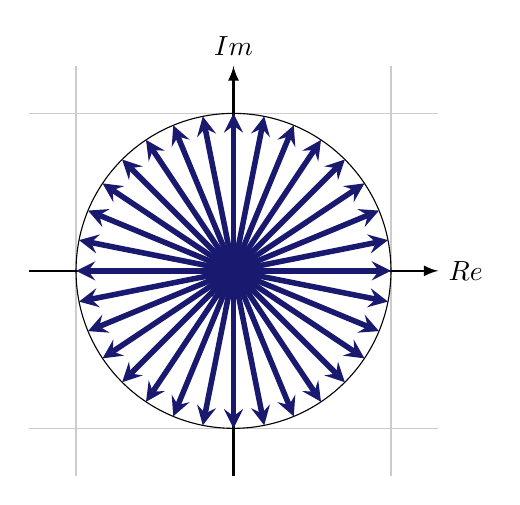
\begin{tikzpicture}[scale=2]
        \def\d{1.3}
        
        \draw[thin,gray!40] (-\d,-\d) grid (\d, \d);
        \draw[thick, ->, >=latex] (-\d,0)--(\d,0) node[right]{\(\mathfrak{Re}\)};
        \draw[thick, ->, >=latex] (0,-\d)--(0,\d) node[above]{\(\mathfrak{Im}\)};
        \draw (0, 0) node[below left] {0};

        \draw (0,0) circle [radius=1];
        
        \def\n{32}

        \foreach \i in {1,...,\n} {
            \draw[line width=2pt, MidnightBlue, -stealth] (0,0)--({cos(360/\n*\i)}, {sin(360/\n*\i)}) node {};
        }
    \end{tikzpicture}
    
    \caption{The roots of unity must lie somewhere on the unit circle.}
    \label{fig:Ch01-unit-circle}
\end{figure}

We want to find the angles \(\theta\) such that if we start at the point \(1\) and then rotate anticlockwise by \(\theta\) radians \(n = 3\) times, we end up back at \(1\).
%
\begin{itemize}
    \item Obviously we can have \(\theta = 0\).
    \item Another obvious solution is \(\theta = 2\pi/3\). If we rotate by this angle \(3\) times, we will have completed a full \(2\pi\) radians, bringing us back to the initial point.
    \item Moreover, we can also have \(\theta = 4\pi/3\). Rotating by this angle \(3\) times creates a total rotation of \(4\pi\) radians (i.e. 2 full cycles), bringing us once again back to the starting point.
    \item Continuing this pattern, it appears that \(\theta = 6\pi/3\) is also a solution. However, this is in fact the same as \(\theta = 0\), since angles differing by \(2\pi\) are considered equivalent. The same applies for \(\theta = 8\pi/3\) (equivalent to \(2\pi/3\)), \(\theta = 10\pi/3\) (equivalent to \(4\pi/3\)), and so on.
\end{itemize}

\begin{figure}[H]
    \centering

    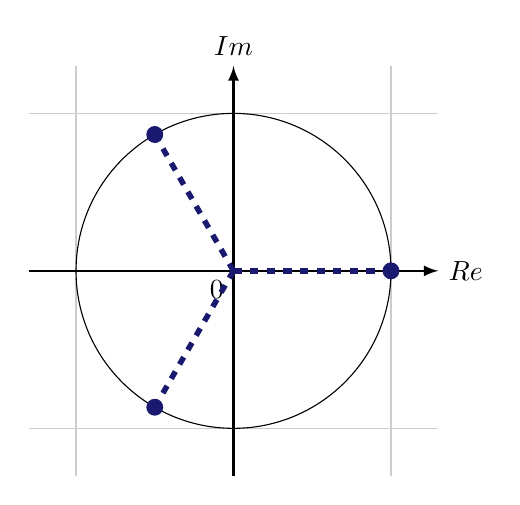
\begin{tikzpicture}[scale=2]
        \def\d{1.3}
        
        \draw[thin,gray!40] (-\d,-\d) grid (\d, \d);
        \draw[thick, ->, >=latex] (-\d,0)--(\d,0) node[right]{\(\mathfrak{Re}\)};
        \draw[thick, ->, >=latex] (0,-\d)--(0,\d) node[above]{\(\mathfrak{Im}\)};
        \draw (0, 0) node[below left] {0};

        \draw (0,0) circle [radius=1];
        
        \def\n{3}

        \foreach \i in {1,...,\n} {
            \filldraw[MidnightBlue] ({cos(360/\n*\i)}, {sin(360/\n*\i)}) circle [radius=0.05];

            \draw[line width=2pt, MidnightBlue, dashed] (0,0)--({cos(360/\n*\i)}, {sin(360/\n*\i)}) node {};
        }
    \end{tikzpicture}
    
    \caption{The third roots of unity.}
    \label{fig:Ch01-3rd-roots-of-unity}
\end{figure}

This resolves the above paradox --- we were right in thinking that the possible values of \(\theta\) are given by
%
\[\theta = \frac{2k\pi}{n}\]
%
or
%
\[\theta \in \left\{\cdots,\; -3\cdot\frac{2\pi}{n},\; -2\cdot\frac{2\pi}{n},\; -\frac{2\pi}{n},\; 0,\; \frac{2\pi}{n},\; 2\cdot \frac{2\pi}{n},\; 3\cdot\frac{2\pi}{n},\; \cdots\right\}\]
%
but these solutions are not all distinct. To make sure we only count distinct solutions, we impose the range \(0 \leq k < n\), giving us
%
\begin{equation}
    \theta = \frac{2k\pi}{n} \tag{\(k \in \mathbb{N}\) and \(k < n\)}
\end{equation}
%
or
%
\[\theta \in \left\{0,\; \frac{2\pi}{n},\; 2\cdot \frac{2\pi}{n},\; 3\cdot\frac{2\pi}{n},\; \cdots ,\; (n-1) \cdot\frac{2\pi}{n}\right\}\text{.}\]
%
This yields the solutions
%
\begin{equation}
    z = 1\times e^{\frac{2k\pi}{n}i} = e^{\frac{2k\pi}{n}i} \tag{\(k \in \mathbb{N}\) and \(k < n\)}
\end{equation}
or
%
\[z \in \left\{0,\; e^{\frac{2\pi}{n}i},\; e^{\frac{4\pi}{n}i},\; \cdots ,\; e^{\frac{2(n-1)\pi}{n}i}\right\}\text{.}\]





